\subsection*{Visualzación de datos}

En la figura \ref{fig:data_2d} se visualizan los datos de varianza, skewness y curtosis por medio de planos.

\begin{figure}[H]
    \centering
    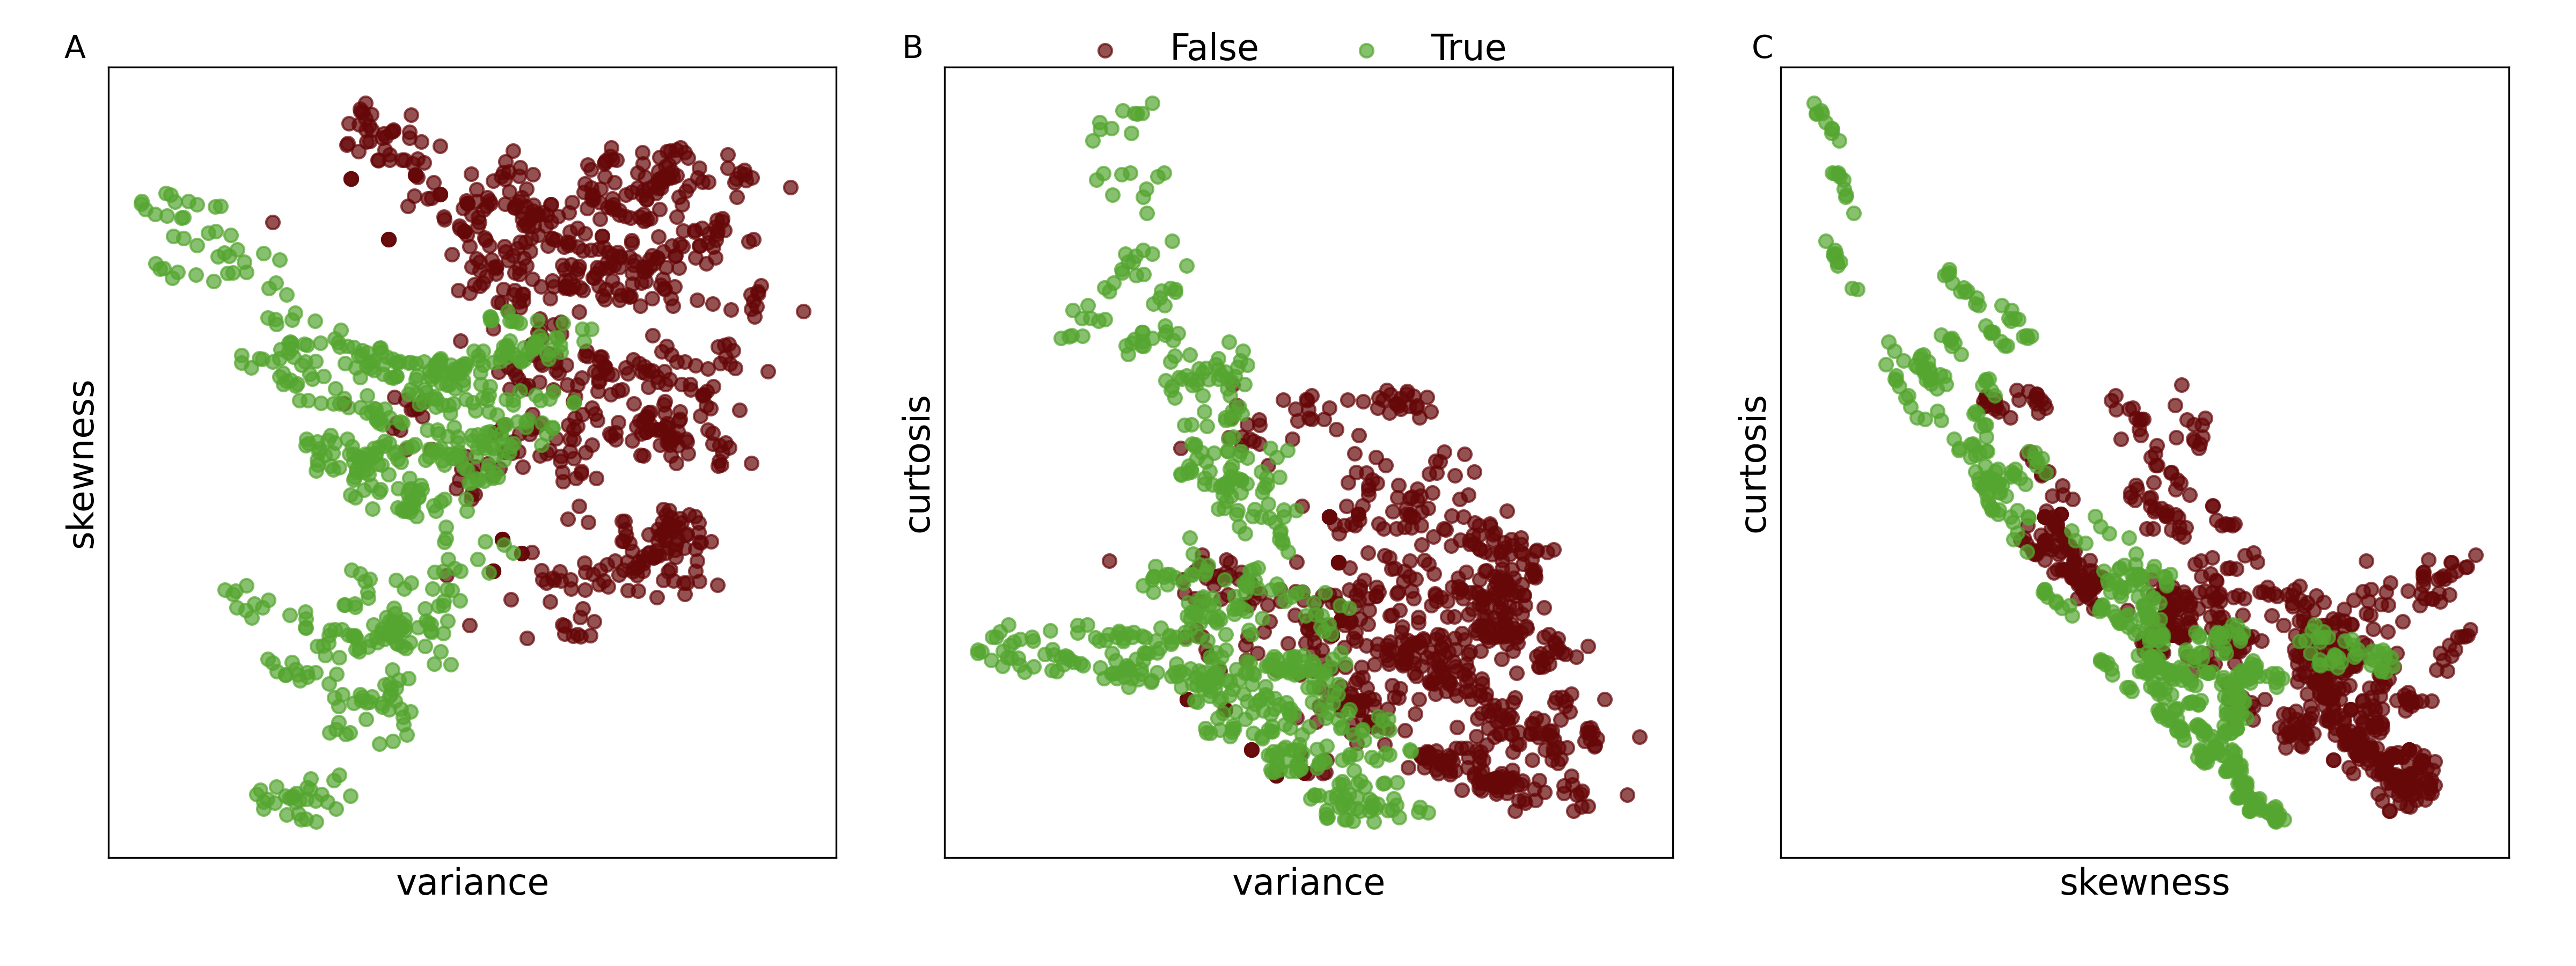
\includegraphics[width=16cm]{Graphics/Problema_04/plot_2D.png}
    \caption{Visualización por planos de los datos de varianza, skewness y curtosis.}
    \label{fig:data_2d}
\end{figure}

La configuración donde se obtiene una mayor diferencia entre cada conjunto de billetes es en el plano de la varianza y la curtosis. En la figura \ref{fig:data_3d} se visualizan los datos usando cada característica para los planos. En esta visualización se logra apreciar de mejor manera que existe una separación entre los dos tipos de billetes.

\begin{figure}[H]
    \centering
    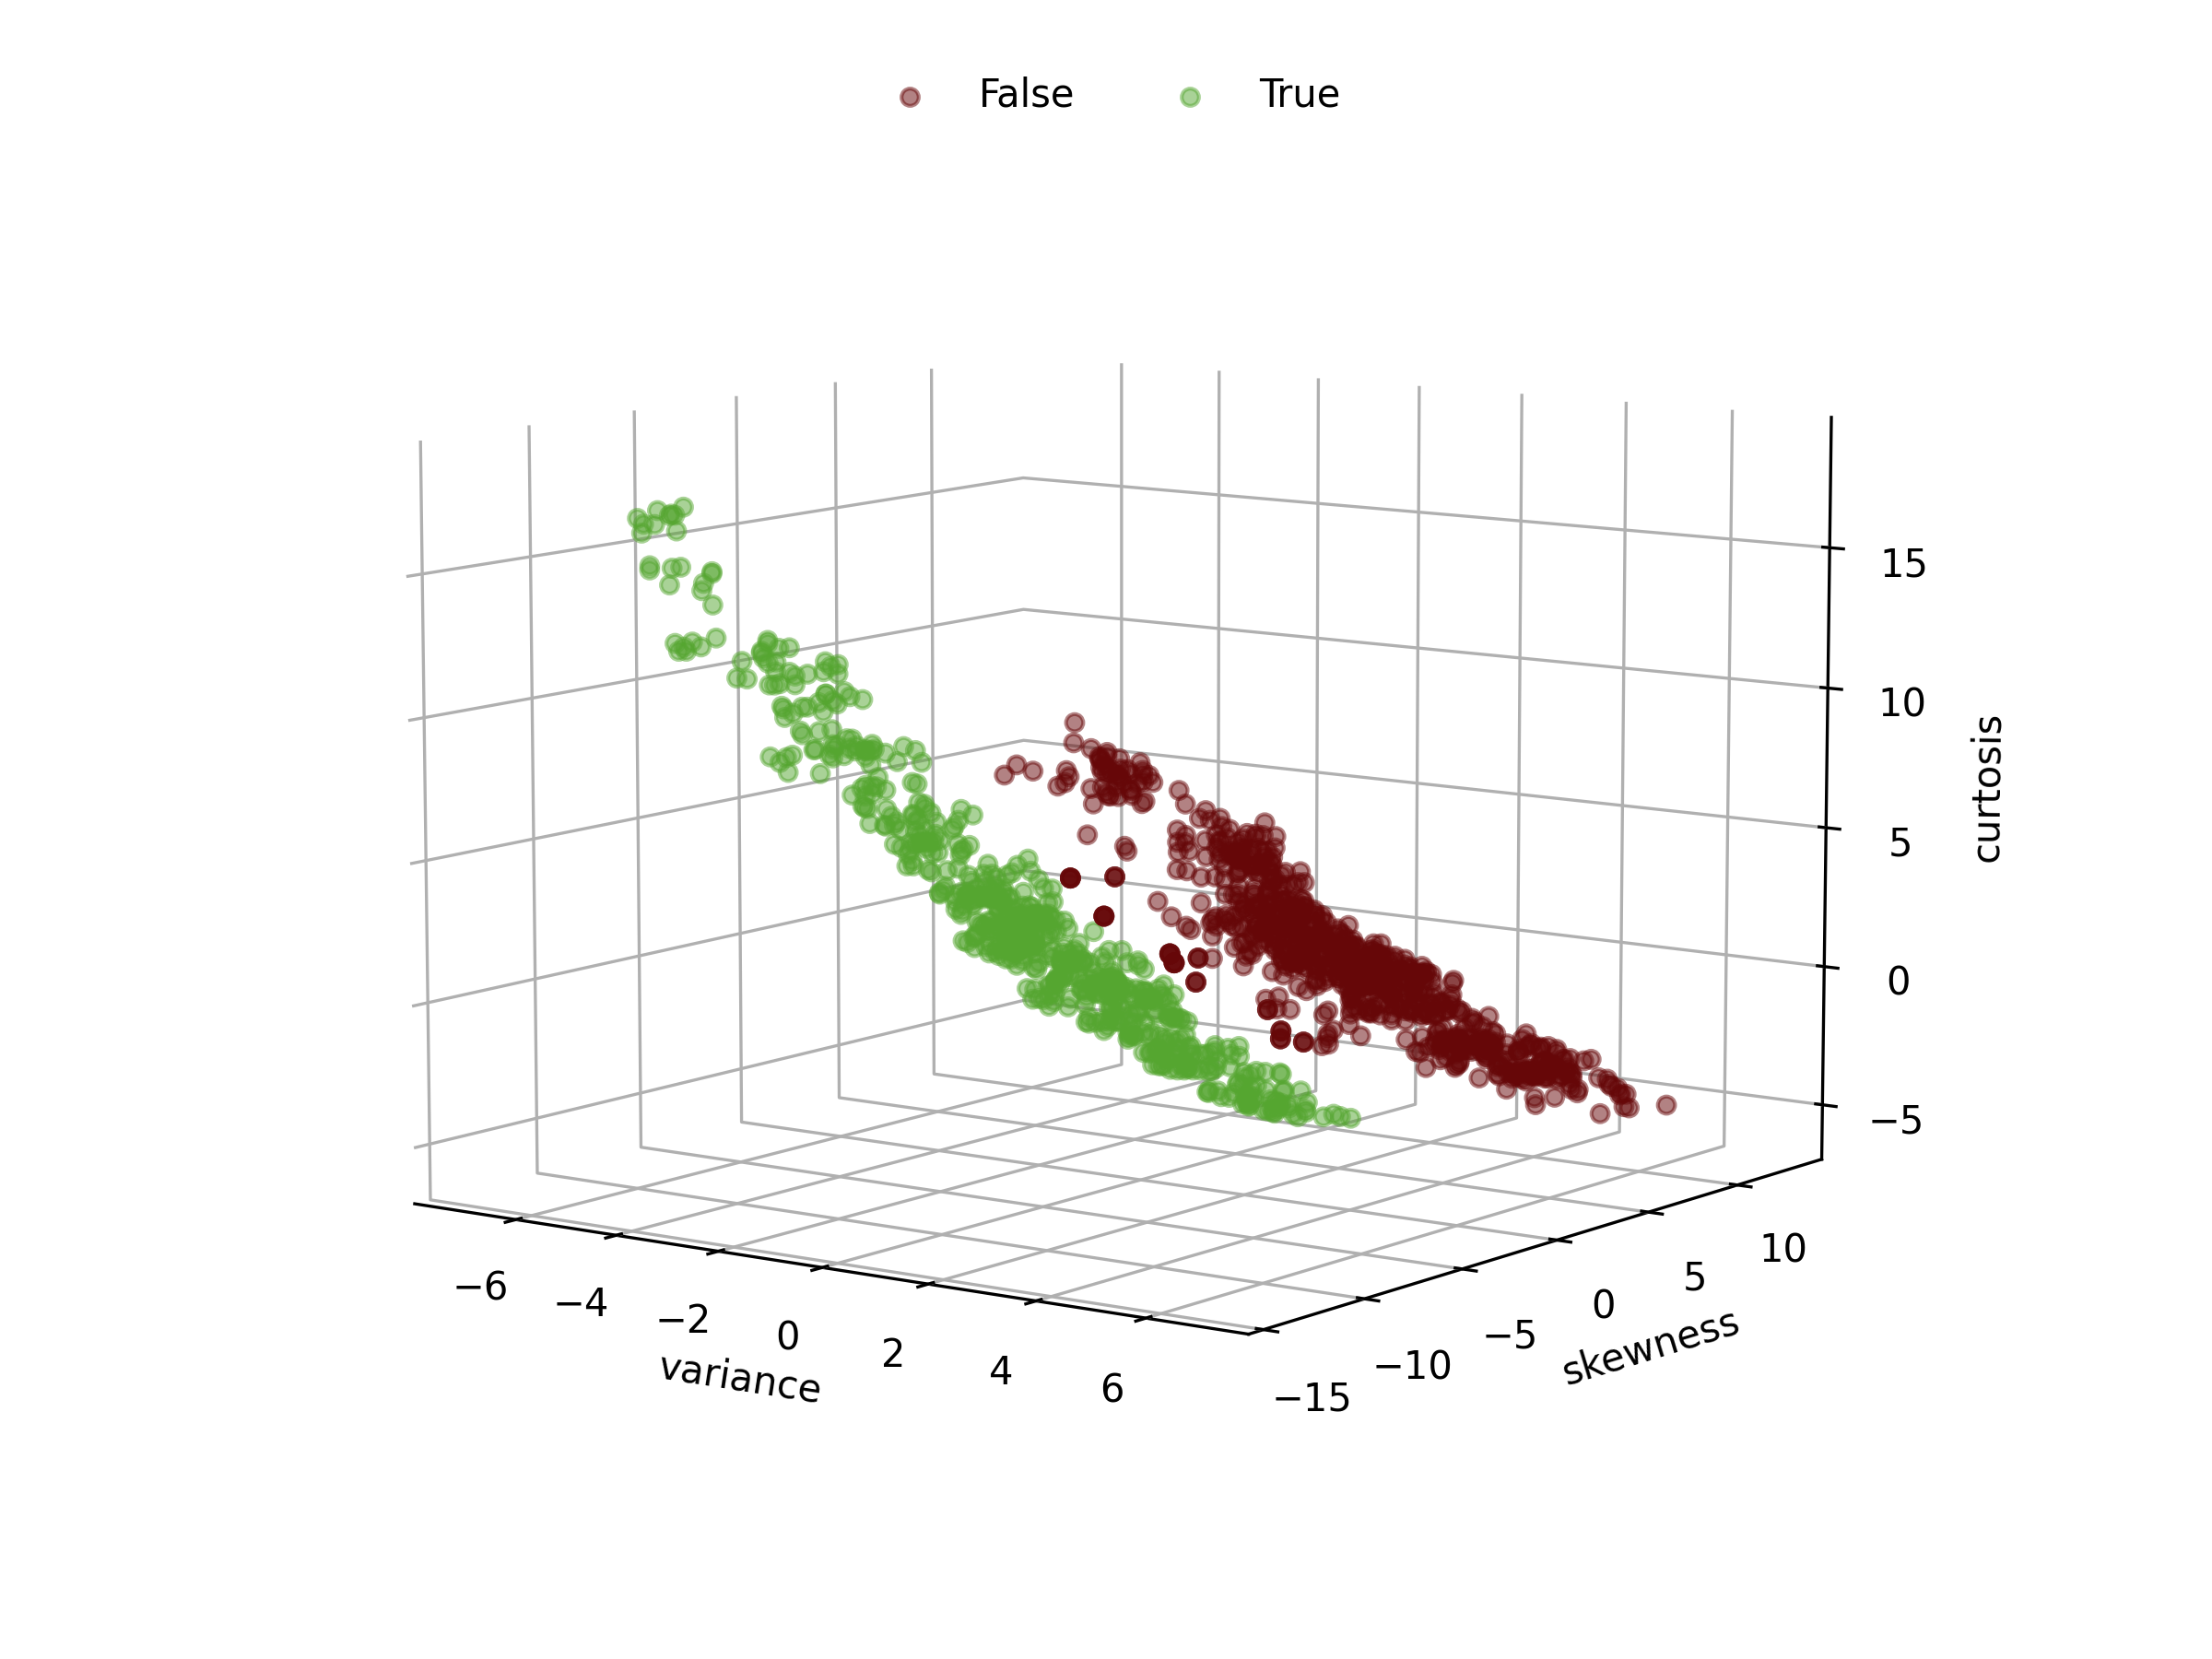
\includegraphics[width=16cm]{Graphics/Problema_04/plot_3D.png}
    \caption{Representación gráfica de los datos usando cada característica como un plano.}
    \label{fig:data_3d}
\end{figure}

Sea $X$ una matriz con las caracteristicas de cada billete donde $X\in R^{n\times 3}$ donde $n$ es el número de billetes caracterizados. Se utilizo la matriz $XX^T$ para iniciar el método de PCA con kernel lineal para obtener un conjunto de datos de dimensión $n\times 3$. En la figura \ref{fig:pca_2d} se visualizan las tres componentes principales obtenidas usando las combinaciones posibles en un plano bidimensional.

\begin{figure}[H]
    \centering
    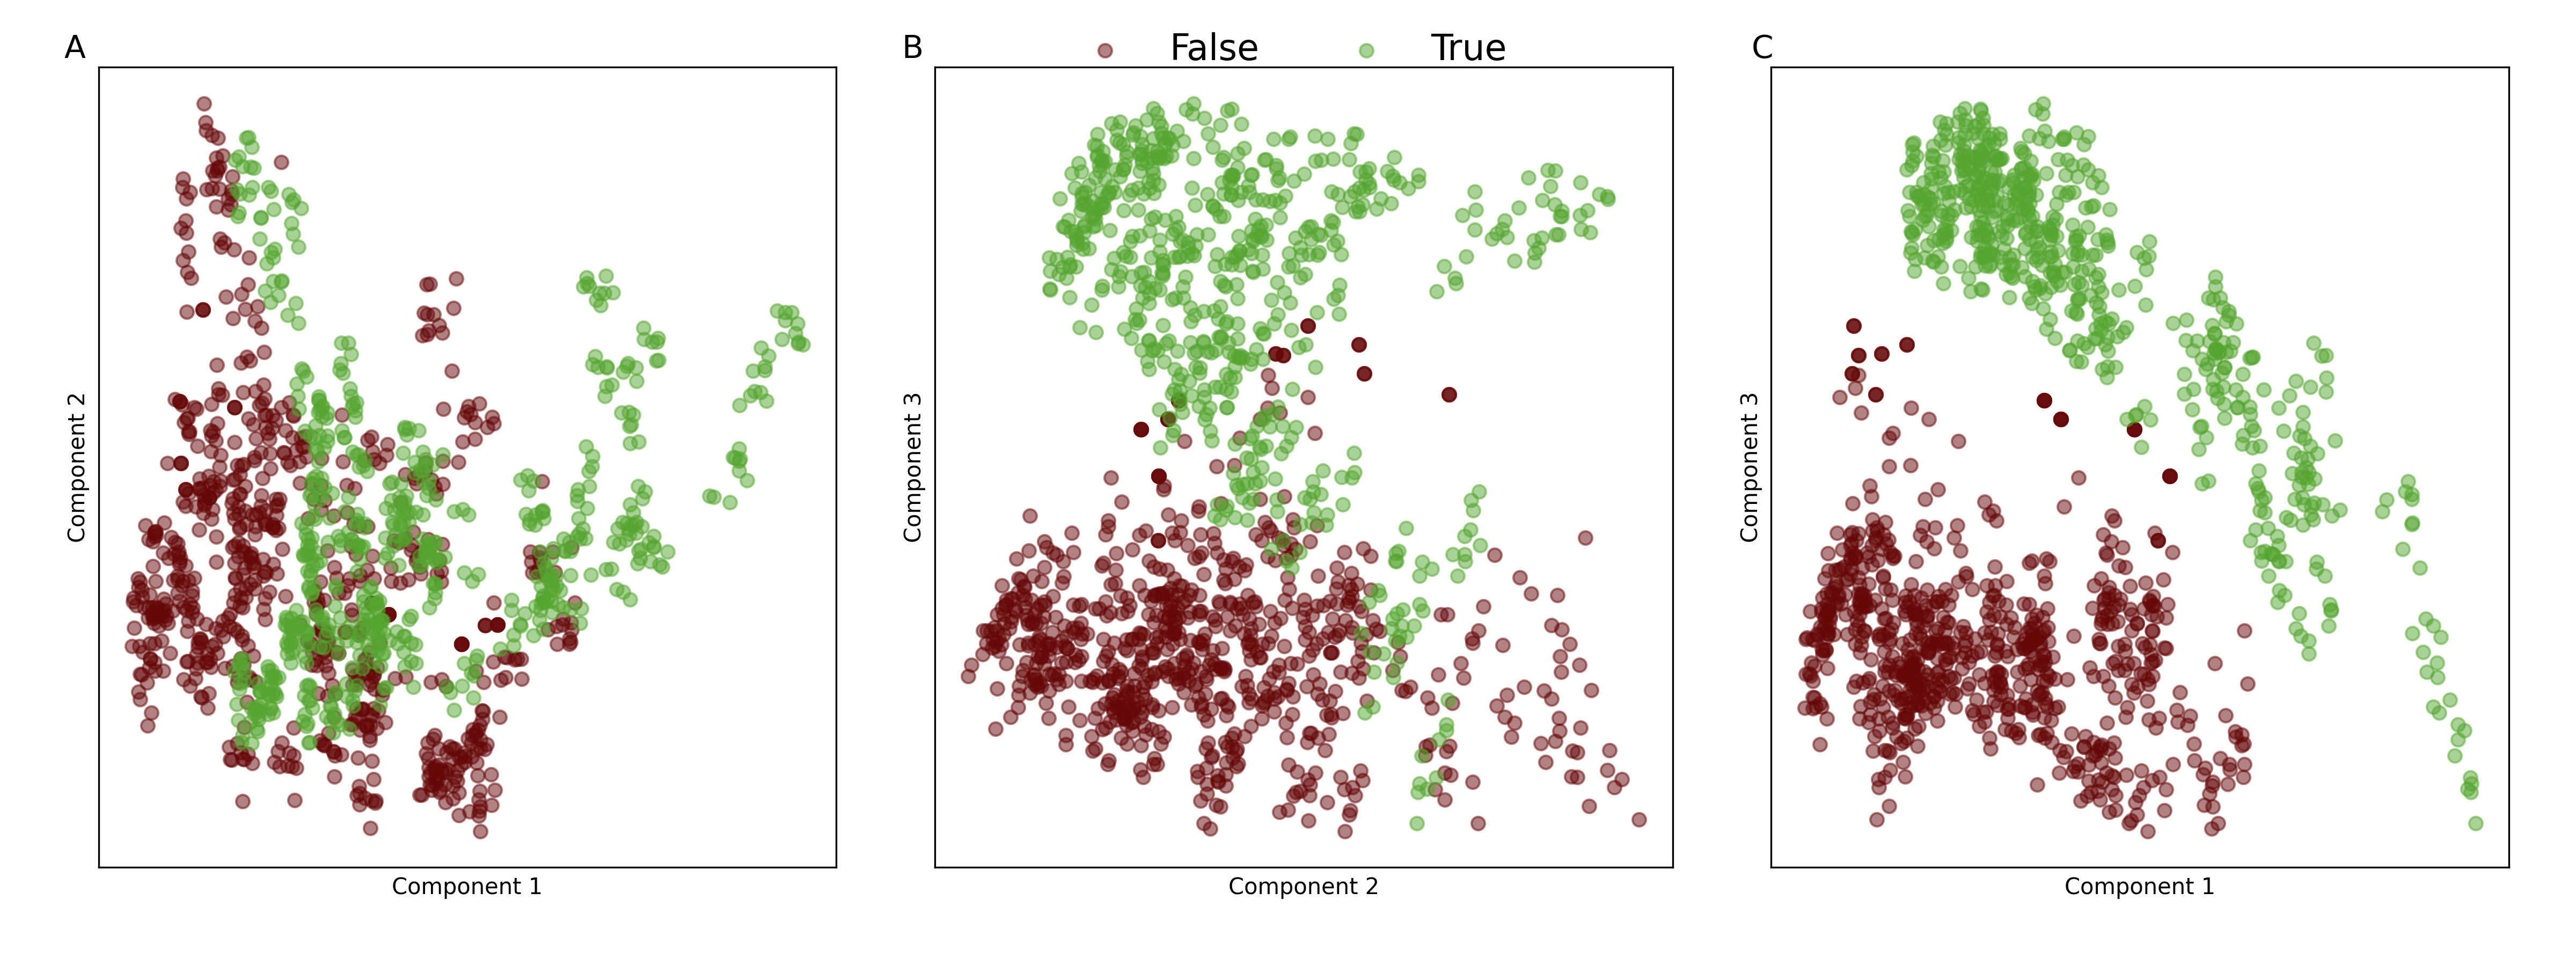
\includegraphics[width=16cm]{Graphics/Problema_04/PCA_2D.png}
    \caption{Representación gráfica de las tres componentes principales obtenidas de PCA usando la matriz $XX^T$.}
    \label{fig:pca_2d}
\end{figure}

Con esta representación se observa que existe una mayor distinción cuando la primer y tercer componentes son usadas como planos. En la figura \ref{fig:pca_3d} se visualizan las tres componentes obtenidas del método de PCA, cada componente usando un plano.

\begin{figure}[H]
    \centering
    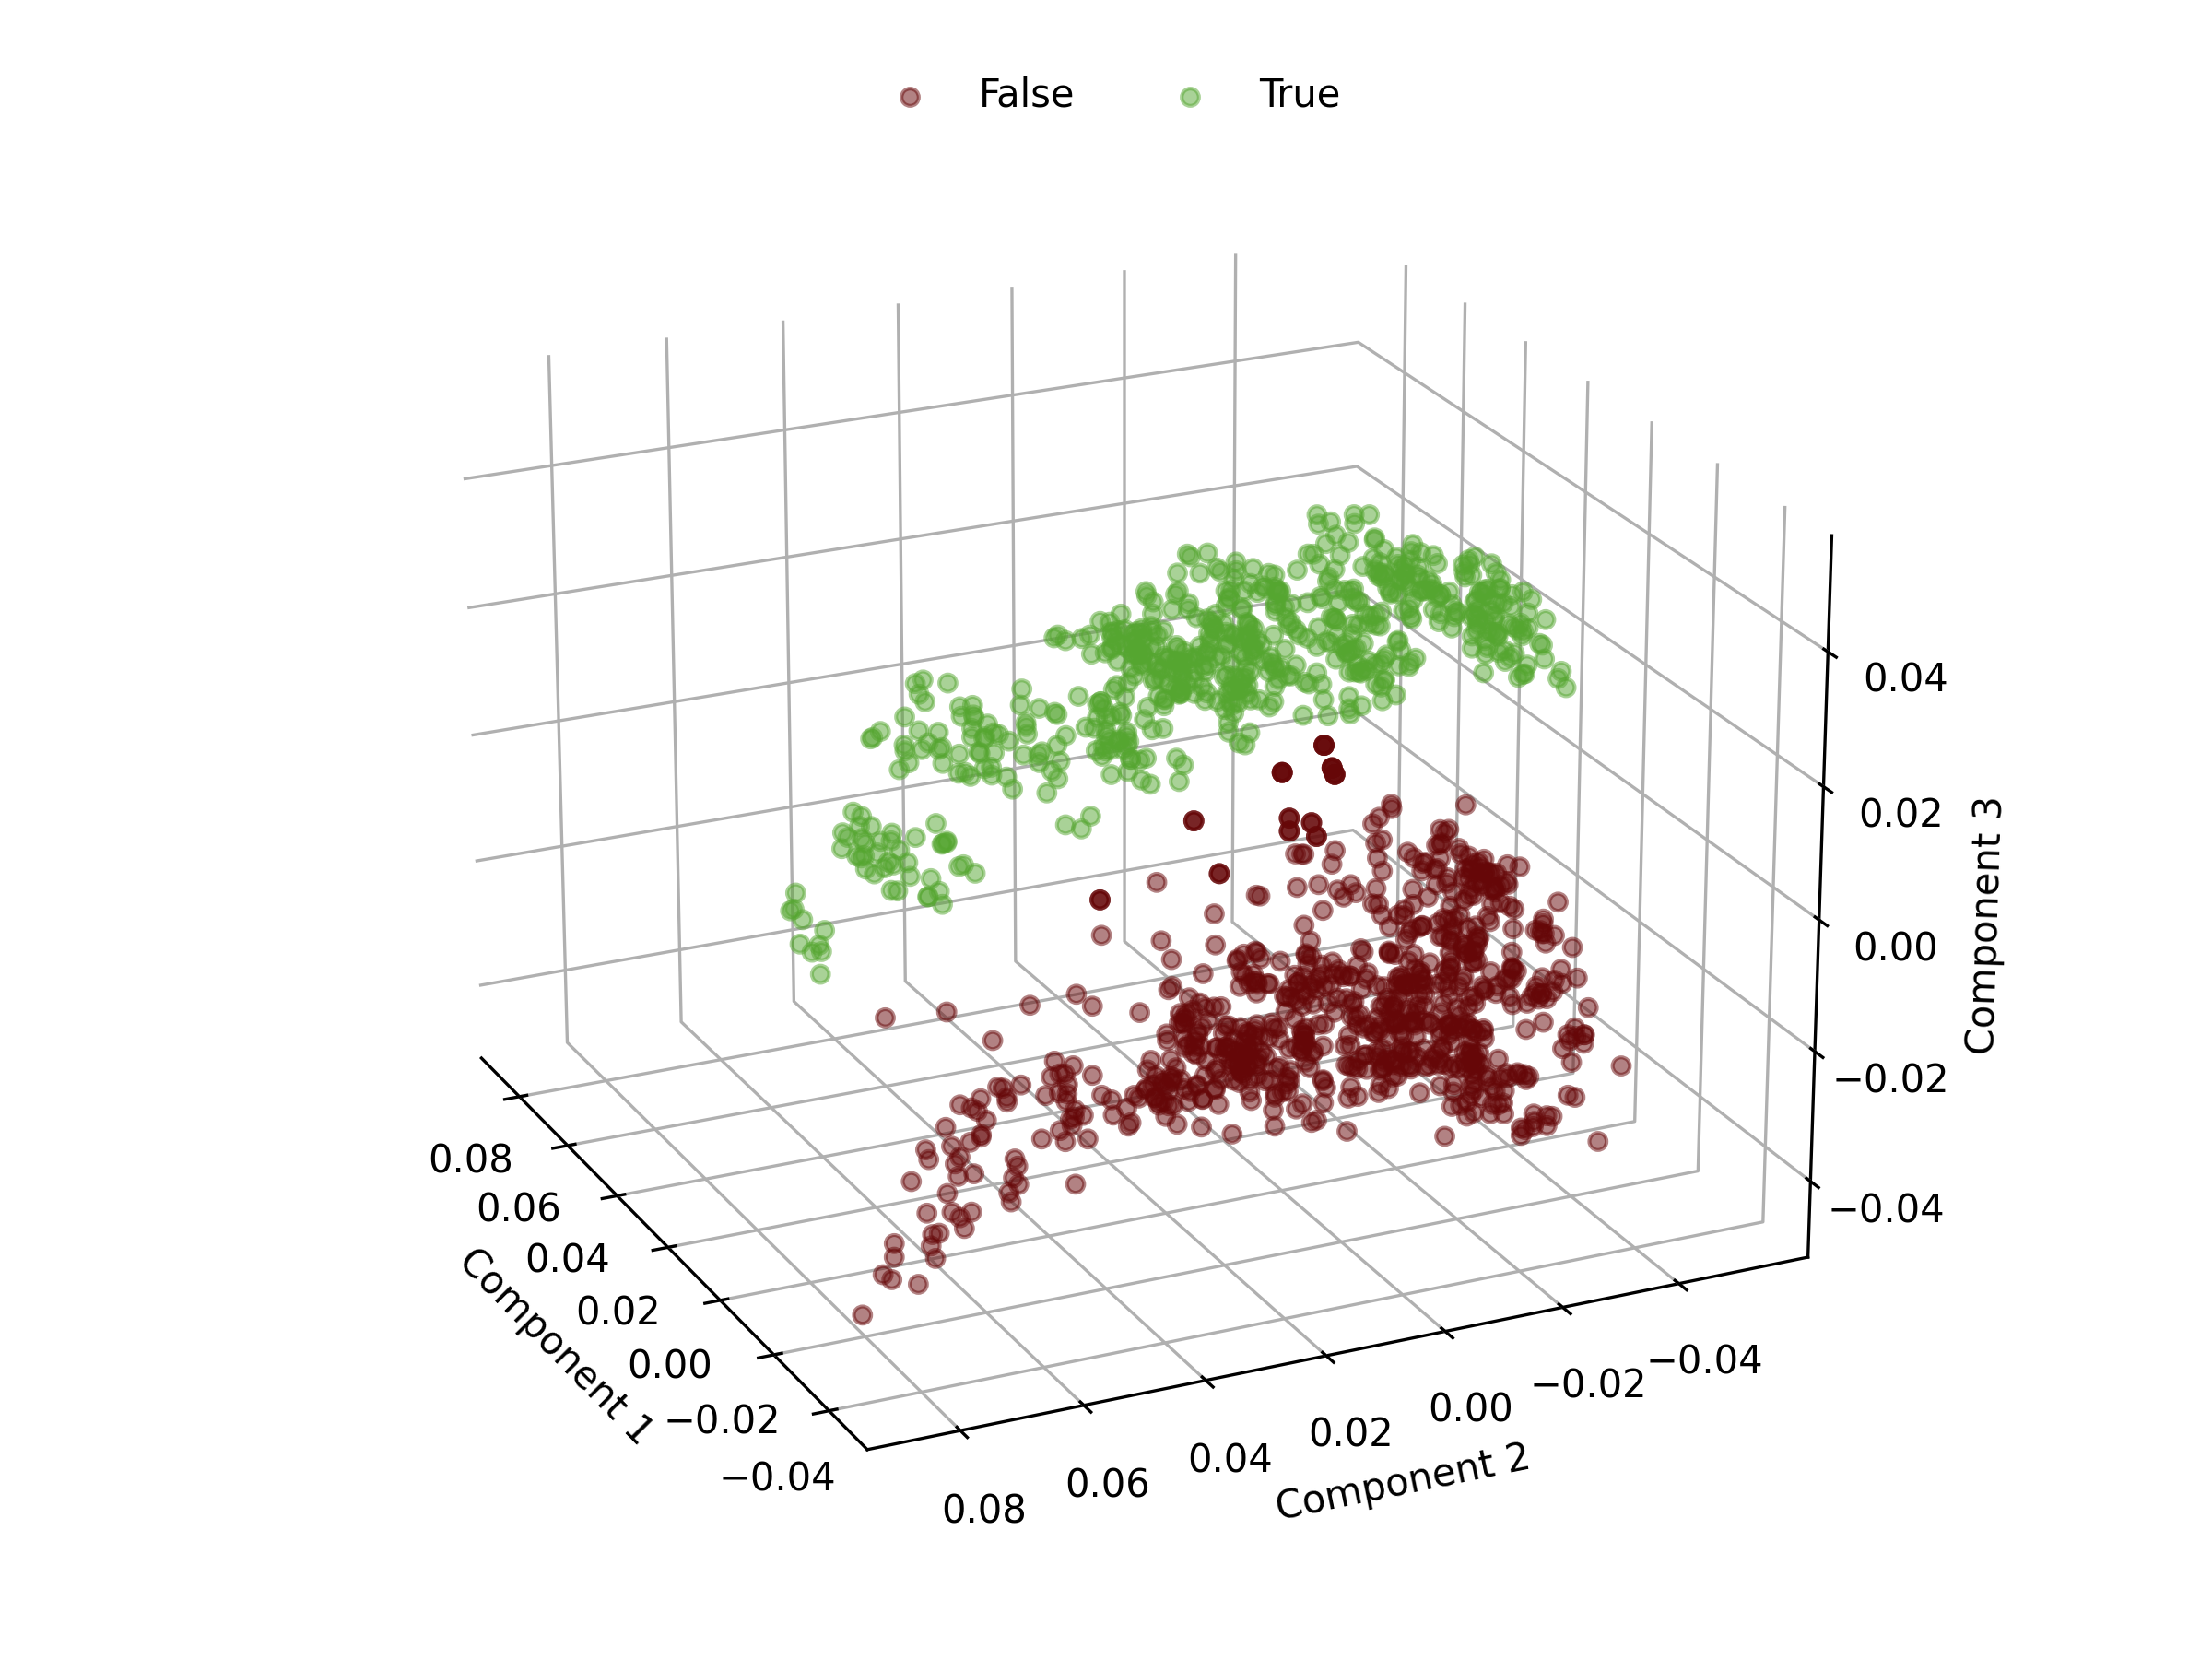
\includegraphics[width=16cm]{Graphics/Problema_04/PCA_3D.png}
    \caption{Representación gráfica de las tres componentes principales obtenidas de PCA usando cada componente como un plano.}
    \label{fig:pca_3d}
\end{figure}

Con esta representación se obtiene de igual manera una distinción entre cada conjutno de billetes. En comparación con la figura \ref{fig:data_3d}, se observa una mayor disperción en los datos.

Para el método de SVM se usaron el kernel lineal, polinomial, rbf y sigmoide. En la tabla \ref{table:parameters} se encuentean los parámetos de cada kernel usado.


\begin{table}[H]
    \centering
    \begin{tabular}{cccc} \hline
        Kernel     & Grado & $\gamma$              & $r$ \\ \hline
        Lineal     & -     & -                     & -   \\
        Polinomial & 3     & $\frac{1}{n\sigma^2}$ & 0   \\
        RBF        & -     & $\frac{1}{n\sigma^2}$ & -   \\
        Sigmoide   & -     & $\frac{1}{n\sigma^2}$ & 0   \\ \hline
    \end{tabular}
    \caption{Parámetros usados para cada kernel. El simbolo $-$ indica que no es necesario el parámetro en el kernel.}
    \label{table:parameters}
\end{table}


Se realizo una partición del conjunto de datos $X$. En esta partición de considero el 90\% como datos de entrenamiento y 10\% como datos de validación. Con los datos de validación se obtuvo un puntaje de precisión. En la tabla \ref{table:data_2d} se encuentran los resultados de aplicar SVM y los datos $X$ como se muestran en la figura \ref{fig:data_2d}.

\begin{table}[H]
    \centering
    \begin{tabular}{lcccc} \hline
        Figura & Lineal & Polinomial & RBF   & Sigmoide \\ \hline
        A      & 0.674  & 0.645      & 0.819 & 0.558    \\
        B      & 0.927  & 0.906      & 0.899 & 0.811    \\
        C      & 0.978  & 1.000      & 1.000 & 0.877    \\ \hline
    \end{tabular}
    \caption{}
    \label{table:data_2d}
\end{table}

Estos resultados pueden ser visualizados en la figura \ref{fig:svm_data}.

Con los datos obtenidos con PCA se obtuvieron los puntajes de precisión mostrados en la tabla \ref{table:pca_2d}.

\begin{table}[H]
    \centering
    \begin{tabular}{lcccc} \hline
        Figura & Lineal & Polinomial & RBF   & Sigmoide \\ \hline
        A      & 0.601  & 0.754      & 0.760 & 0.565    \\
        B      & 0.927  & 0.848      & 0.920 & 0.826    \\
        C      & 0.964  & 1.000      & 1.000 & 0.862    \\ \hline
    \end{tabular}
    \caption{}
    \label{table:pca_2d}
\end{table}

Estos resultados pueden ser visualizados en la figura \ref{fig:svm_pca}.

Tratando a los conjuntos de datos como en las figuras \ref{fig:data_3d} y \ref{fig:pca_3d}, se obtuvieron los puntajes mostrados en la tabla \ref{table:results_3d}.

\begin{table}[H]
    \centering
    \begin{tabular}{lcccc} \hline
        Datos      & Lineal   & Polinomial & RBF & Sigmoide \\ \hline
        Originales & 0.992754 & 0.992754   & 1.0 & 0.73913  \\
        PCA        & 1.0      & 1.0        & 1.0 & 0.876812 \\ \hline
    \end{tabular}
    \caption{}
    \label{table:results_3d}
\end{table}

\pagebreak

\begin{figure}[H]
    \centering
    \includegraphics[width=16cm]{Graphics/Problema_04/SVM_data.png}
    \caption{}
    \label{fig:svm_data}
\end{figure}

\pagebreak

\begin{figure}[H]
    \centering
    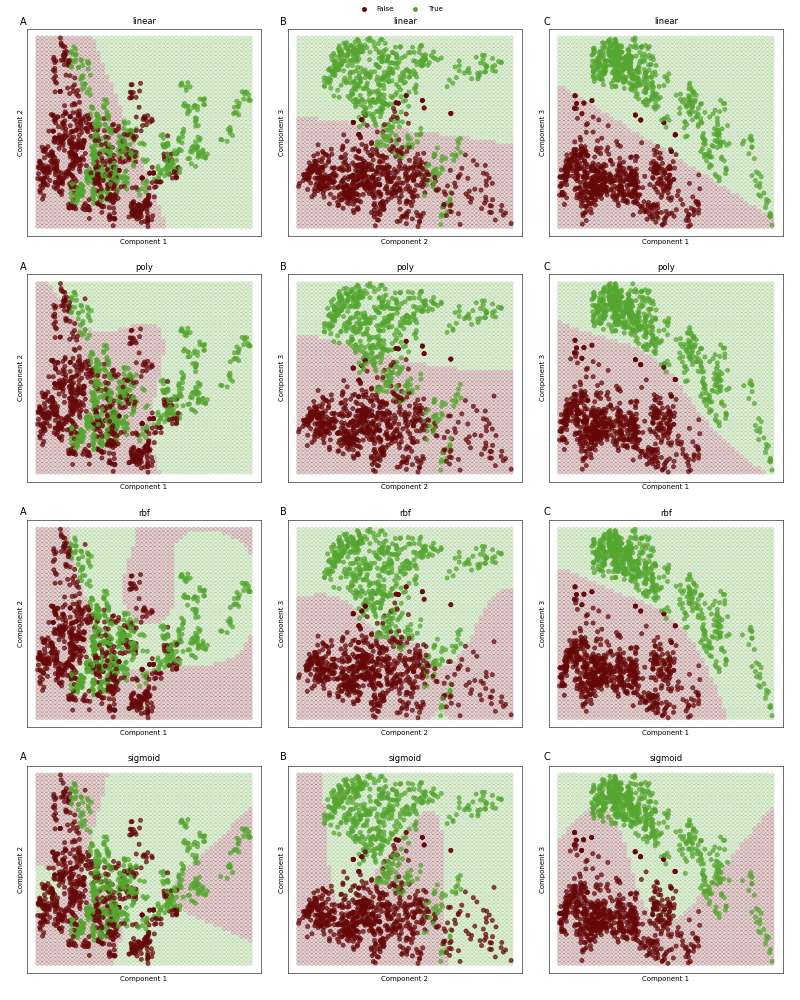
\includegraphics[width=16cm]{Graphics/Problema_04/SVM_PCA.png}
    \caption{}
    \label{fig:svm_pca}
\end{figure}